
%%%%%%%%%%%%%%%%%%%%%%%%%%%%%%%%%%%%%%%%%%%%%%%%%%%%%%%%
% LaTex Template for proposals within the              %
% DFG Research Unit Program                            %         
%Planet Formation Witnesses and Probes: Transition Discs
% August 2016                                            %                           
%                                                      %
%%%%%%%%%%%%%%%%%%%%%%%%%%%%%%%%%%%%%%%%%%%%%%%%%%%%%%%%
%
% 
%
% This template may be used to prepare proposals in latex.
%
%
% The project description, including publication list, should be no more than 20 pages
% in length. It should be self-explanatory and not require reviewers to read the 
% literature that is quoted or enclosed.

\documentclass[10pt,fleqn,twoside]{article}

%%%% USE ARIAL FONT %%%%%%%%%%%%%%%%%%%%%%%%%%%%%%%%%%%%%%%%%%%%%%%%%%%%%%
\usepackage{helvet}
\renewcommand\familydefault{phv}

%%%% INCLUDE NECESSARY PACKAGES %%%%%%%%%%%%%%%%%%%%%%%%%%%%%%%%%%%%%%%%%%
%\usepackage{babel}
\usepackage[UKenglish]{babel}
\usepackage{amsmath}
\usepackage{amssymb}
\usepackage{fancyhdr}
\usepackage{natbib}
\usepackage{ae,aecompl}
\usepackage{graphicx}
\usepackage{palatino}
\usepackage[T1]{fontenc}
\usepackage[right]{eurosym}
\usepackage{rotating}
\usepackage{epsf}
\usepackage{setspace}
\usepackage{xspace}
\usepackage{multicol}
\usepackage{siunitx}
%\usepackage{caption}

\usepackage{sfmath}

\usepackage[utf8]{inputenc}

% ========= hyperref & Colors & Links ===========
\usepackage[usenames,dvipsnames]{xcolor}
%\usepackage[breaklinks]{hyperref}
\usepackage{hyperref}
\addto\extrasUKenglish{%
\def\sectionautorefname{Section}%
\def\subsectionautorefname{Section}%
\def\subsubsectionautorefname{Section}%
\def\paragraphautorefname{Section}%
}
\usepackage[all]{hypcap} % fixes links to floats
\usepackage{aas_macros}  %
\setlength{\bibsep}{-0.5pt}

% ========= highlighting important parts of the proposal ===========
\definecolor{HighLight}{rgb}{0.9,0.3,0.0}
%\newenvironment{highlight}{\color{blue}\itshape}{\ignorespacesafterend}
%\newenvironment{highlight}{\color{RedOrange}\itshape}{\ignorespacesafterend}
%\newenvironment{highlight}{\color{RedOrange}\bfseries}{\ignorespacesafterend}
%\newenvironment{highlight}{\color{BrickRed}\bfseries\itshape}{\ignorespacesafterend}
%\newenvironment{highlight}{\color{BrickRed}\bfseries}{\ignorespacesafterend}
%\newenvironment{highlight}{\color{HighLight}\bfseries}{\ignorespacesafterend}
\newenvironment{highlight}{\color{HighLight}}{\ignorespacesafterend}
\newenvironment{missingenv}{\color{red}}{\ignorespacesafterend}

\definecolor{Emphasize}{rgb}{0.0,0.5,0.0}
\newenvironment{Emphasize}{\color{Emphasize}\itshape}{\ignorespacesafterend}


% strike through comments: to turn them off, uncomment the renewcommands below
\usepackage{soul}
\setstcolor{red}

% ========= Commands specially for the forschergruppe =========

\newcommand{\todo}[1]{\textcolor{red}{\bf #1}}
\newcommand\connect[1]{{\color{OliveGreen} #1}}

%%%% CAPTION LAYOUT %%%%%%%%%%%%%%%%%%%%%%%%%%%%%%%%%%%%%%%%%%%%%%%%%%%%%

\usepackage[font={small}]{caption}

%%%% PAGE LAYOUT %%%%%%%%%%%%%%%%%%%%%%%%%%%%%%%%%%%%%%%%%%%%%%%%%%%%%%%%%
\setlength{\textheight}{22cm}
\setlength{\topmargin}{-1.2cm}
\setlength{\textwidth}{15.6cm}
\setlength{\oddsidemargin}{0.0cm}
\setlength{\evensidemargin}{0.0cm}
\setlength{\mathindent}{1.5cm}
\setlength{\parindent}{0.0cm}
\setlength{\parskip}{0.08cm}

%%%% PAGE HEADER %%%%%%%%%%%%%%%%%%%%%%%%%%%%%%%%%%%%%%%%%%%%%%%%%%%%%%%%%%
\pagestyle{fancy}
\fancyhead[RE,RO]{}
\fancyfoot[RO]{\thepage}
\fancyfoot[LE]{\thepage}
\fancyfoot[CE,CO]{}

%%% FONTS FOR THE TITLE PAGE %%%%%%%%%%%%%%%%%%%%%%%%%%%%%%%%%%%%%%%%%%%%%%
\newfont{\tpfonta}{cmssbx10 scaled 1600}
\newfont{\tpfontb}{cmssbx10 scaled 3200}

%%%% COLOR DEFINITIONS %%%%%%%%%%%%%%%%%%%%%%%%%%%%%%%%%%%%
\definecolor{blue} {rgb} {0.25,0.25,0.75}

%%%% ADDITONAL EMPHASIS %%%%%%%%%%%%%%%%%%%%%%%%%%%%%%%%%%%
\newcommand{\cem}{\color{blue}}
\newcommand{\eem}{\sl\color{blue}}

%%%% BIBTEX PUNCTUATION %%%%%%%%%%%%%%%%%%%
\bibpunct{(}{)}{;}{a}{}{,} % to follow the A&A style

%%%% SET THE COLOR OF THE (SUB-) SECTION TITLES %%%%%%%%%%% 
\newcommand{\Tcol}{\color{blue}}

%%%% SET THE COLOR OF THE TITLE BOX BACKGROUND %%%%%%%%%%%%
\definecolor{Background}{rgb} {0.62,0.75,0.5}

%%%%%%%%%%%%%% REFERENCE SECTION NAME %%%%%%%%%%%%%%%%%%%%
\renewcommand\refname{\Tcol 9. Bibliography}

%%%%%%%%%%%%%% NICER PROJECT REFERENCES %%%%%%%%%%%%%%%%%%%

\newenvironment{literature}%
 {\begin{multicols}{2}\begin{scriptsize}\begin{list}{}{%
   \setlength{\topsep}{0em}%
   \setlength{\parskip}{0em}%
   \setlength{\parsep}{0em}%
   \setlength{\itemsep}{0em}%
   \setlength{\rightmargin}{0em}%
   \setlength{\leftmargin}{2em}%
   \setlength{\itemindent}{-2em}}}%
 {\end{list}\end{scriptsize}\end{multicols}}

%
% ...A compact itemize environment
%
\newenvironment{compactitemize}%
 {\begin{list}{$\bullet$}{%
   \setlength{\topsep}{0em}%
   \setlength{\parskip}{0em}%
   \setlength{\parsep}{0em}%
   \setlength{\itemsep}{0.0\baselineskip}%
   \setlength{\rightmargin}{0em}%
   \setlength{\leftmargin}{2.0em}%
   \setlength{\labelsep}{0.5em}%
   \setlength{\labelwidth}{1em}%
}}
 {\end{list}}

\newcounter{qcounter}
\newenvironment{compactenumerate}%
 {\begin{list}{\arabic{qcounter})~}{\usecounter{qcounter}%
   \setlength{\topsep}{0em}%
   \setlength{\parskip}{0em}%
   \setlength{\parsep}{0em}%
   \setlength{\itemsep}{0.0\baselineskip}%
   \setlength{\rightmargin}{0em}%
   \setlength{\leftmargin}{2.0em}%
   \setlength{\labelsep}{0.5em}%
   \setlength{\labelwidth}{1em}%
}}
 {\end{list}}

%%%% EXPLANATION FOR THE CONNECT COLOR %%%%%%%%%%% 
\newcommand{\footexplainconnect}{\footnote{The text highlighted in \connect{green} refers to the connection of this project to other projects of this Research Unit.}}
 
%%%%%%%%%%%%%%%%%% NICER REFERENCES %%%%%%%%%%%%%%%%%%%

%\usepackage[capitalise,nameinlink]{cleveref}
\newcommand{\cref}[1]{\autoref{#1}}

%%%%%%%%%%%%%%%%%% COLOR THE SECTION NUMBERS %%%%%%%%%%%%%%%%%

\makeatletter
\renewcommand\@seccntformat[1]{\color{blue} {\csname the#1\endcsname}\hspace{0.5em}}
\makeatother
\renewcommand\thesection{\arabic{section}.}
\renewcommand\thesubsection{\arabic{section}.\arabic{subsection}}

%%%%% color sections
\usepackage{sectsty}
\allsectionsfont{\color{blue}}


%%%% CHANGE THE APPEARANCE OF THE \PARAGRAPH COMMAND  %%%%%%%%%%%%%%%%%%%%%%%%%%%%%%%
\makeatletter
\renewcommand\paragraph{\@startsection{paragraph}{4}{\z@}%
            {-2.5ex\@plus -1ex \@minus -.25ex}%
            {1.25ex \@plus .25ex}%
            {\normalfont\normalsize\bfseries\Tcol}}
\makeatother
\setcounter{secnumdepth}{4}     % how many sectioning levels to assign numbers to
\setcounter{tocdepth}{4}        % how many sectioning levels to show in ToC

%%%%% set header

\renewcommand{\sectionmark}[1]{\markright{\color{black}#1}}

\newcommand{\caphighlight}[1]{{\bf #1}}



\newcommand{\til}[1]{\todo[color=LimeGreen,inline]{Til: #1}}
\newcommand{\barbara}[1]{\todo[inline]{Barbara: #1}}


\fancyhead[LE,LO]{\slshape
%%%%  Please edit
%
Ercolano \&
Birnstiel: RU Transition Discs project C2}
%
%
%%%%%


\begin{document}


\newpage

%%%% PROJECT DESCRIPTION STARTS HERE %%%%%%%%%%%%%%%%%%%%%%%%%%%%%%%%%%%

\setcounter{page}{1}

\centerline{\huge\bf\Tcol
%
%
%
%
%%%%  Please edit
%
 Project C2:}
\vspace{1em}

\centerline{\LARGE\bf\Tcol Gone with the wind:}\vspace{0.3em}
\centerline{\LARGE\bf\Tcol Dust entrainment in photoevaporative winds}

%
%%%%
%
%
%
%
\vskip1.0cm

%%%%  Please edit

\noindent{\bf Authors:}\\
\begin{tabular}{ll}
{\textsf{PI:}}                   & B.~Ercolano (LMU) \\
{\textsf{Co-I:}}                & T.~Birnstiel (LMU), C.~Dullemond (Heidelberg)\\
{\textsf{Collaborations:}}      &  James Owen (Princeton, USA),
                                    C.~Dullemond
                                  (Heidelberg), T. Henning (MPIA)\\

\end{tabular}

%%%%  Please edit

\vspace{1em}
\noindent{\bf Requested positions: 1PhD student} \\

\vspace{1em}
\noindent{\bf Abstract:}\\
The search for the smoking gun of disc dispersal via photoevaporative
winds, which destroy discs via the formation of Type 1 TDs,  has until
now failed to identify suitable diagnostics. Quantitative spectroscopy of
YSOs to search for blue-shifted emission lines produced in the wind
relies on an accurate characterisation of the thermochemical
properties of the winds. A central ingredients for the chemical
calculations is the dust content of the wind as micron sized grains
provide the dominant opacity channel in the far-ultraviolet.
Furthermore small particles are important players in the temperature
balance of the gas via the photoelectric process.  

We will use realistic radiation-hydrodynamic models of
photoevaporative winds coupled to dust evolution models for the
underlying grain distribution in the disc, to calculate the dust
entrainment in winds to feed to chemical models. The observability of
the emission and scattering due to the dust grains in winds from edge-on
discs, a potential new diagnostic, will be estimated for current and
upcoming facilities (e.g.\ SPHERE, JWST) both for Herbig
Ae stars and for their fainter T-Tauri counterparts.  

\section{State of the art and preliminary work}
\renewcommand{\leftmark}{\sc State of the Art and preliminary work}

The dispersal of protoplanetary discs plays a crucial role in the
planet formation process, and leads to the formation of Type
1 TDs. While photoevaporation from the central star has been proposed
as the dominant disc-dispersal mechanism around low-mass stars
(e.g.\ Clarke et 2001), to date the only evidence that exists of a
wind detection, via blue-shifted forbidden line emission of mostly
[NeII], [OI] and a number of other optical forbidden lines, which can
be matched with more or less success by photoevaporation models
(e.g.\ Hartigan, Edwards \& Ghandour 1995; Alexander 2008; 
Rigliaco et al.\ 2013; Natta et al.\ 2014; Pascucci \& Sterzik 2009; Schisano, Ercolano \& Guedel 2010; Ercolano
\& Owen 2010, 2016, Simon et al.\ 2016). These lines however  can only probe the wind on very local
scales and they cannot be inverted to obtain mass loss rates, which
are crucial to pin down the dominating mechanism which drives the disc
photoevaporative wind
(i.e.\ EUV, FUV or X-ray - or a combination). Different driving
mechanism induce more or less vigorous mass loss at different disc
radii, which  can have dramatic effect on planet formation, both at
the times of planetesimal assembly and for the later dynamical
evolution of planet(esimal)s (e.g.\ Alexander \& Pascucci 2012;
Ercolano \& Rosotti 2015).   

\connect{Projects B1 \& B2 aim at identifying and using new spectroscopic
diagnostics to qualitatively measure mass loss rate and profile in disc 
winds. In order to achieve these aims a chemical model of the wind will
be constructed in B2 using the wind structures from
radiation-hydrodynamic calculations performed in B1.} Chemistry is
sensitively affected by the dust distribution in the wind and
underlying disc atmosphere, but to date only rough estimates exist
(e.g.\ Owen, Ercolano \& Clarke 2011b; Hutchison et al.\ 2016ab). While
the results of these works are not yet to the stage that they can 
be used in the chemical model, they demonstrate
that a non-negligible population of small grains, which dominate the
opacity in the FUV, are to be expected in the winds. 

Owen, Ercolano \& Clarke (2011b) demonstrated that in the case of
Herbig Ae/Be stars with an EUV-driven wind, the wind selectively entrains
grains of different sizes at different radii resulting in a dust
population that varies spatially and increases with height above the
disc at radii larger than about 10~AU. At near infrared wavelengths
this variable grain population produces a 'wingnut' morphology which
may have already been observed in the case of PDS 144N (Perrin et al.
2006). The work of Owen et al.\ (2011b) could not however reproduce the
colour gradient of the observations, which show redder emission at
larger heights above the disc. Possibly the problem was due to the
fact that the synthetic images were dominated by emission from the
smallest grains entrained in the flow. Grain growth in the underlying
disc, neglected in the
Owen et al.\ (2011b) calculations, is a natural solution to
the colour problem, which needs to be taken into account in future
simulations. 

While it is currently not clear if the PDS 144N observations can be
explained by dust entrainment in a photoevaporative wind, the work of
Owen, Ercolano \& Clarke (2011b) has clearly demonstrated that a
significant amount of small grains (which dominate the opacity in the
FUV) do populate disc winds, hence playing an important part in the
chemistry there and at the base of the flow. 

More recently Hutchison et al.\ (2016ab) investigated the question of
dust entrainment in protoplanetary discs using smoothed particle
hydrodynamics (SPH). While their models are very idealised (non-rotating,
plane-parallel discs), their simulations seem to support most of the
conclusions reported in the semi-analytical work of Owen, Ercolano \&
Clarke (2011b). The Hutschison et al.\ models also only consider an a
EUV-driven wind, in order to simplify the calculations.  

\subsection{Dust-entrainment in winds: modelling strategies}

In this section two approaches to model dust-entrainment in
winds are described in more detail. The limitations of both approaches
are also discussed, thus highlighting the knowledge gap that our
project is aiming to fill. 

\subsubsection{Analytical approach}\label{sec:analytical-approach}

Owen, Ercolano \& Clarke (2011b) post-processed
radiation-hydrodynamical simulations of photoevaporating disc winds
around Herbig Ae/Be stars in order to study the distribution and
observational appearance of dust grains entrained in the wind. Their
approach involved three steps: (i) (radiation)-hydrodynamical
calculations of the photoevaporative wind; (ii) calculation of the
dust profile distribution in the wind; (iii) radiative transfer
calculation of the dust distribution to infer the observational
appearance. 

As the work of Owen, Ercolano \& Clarke (2011b) was motivated by the
observations of several edge-on discs around Herbig stars, which
showed extended emission above and below their midplane at NIR
wavelengths (e.g.\ Padgett et al.\ 1999, Perrin et al.\ 2006), these
authors focussed in step (i)  on EUV-driven winds (e.g.\ Hollenbach et al.\ 1994;
Font et al.\ 2004; Alexander, Clarke \& Pringle 2006a,b). Indeed Herbig
stars have generally a much lower X-ray luminosity relative to their
bolometric luminosity, compared to T-Tauri stars, raising questions on
what the driving radiation may be for these intermediate mass stars. For
that reason Owen, Ercolano \& Clarke (2011b) chose to adopt the
hydrodynamic EUV wind solution of Font et al.\ (2004), which is simple and
scalable, hence allowing them to investigate a wider range of
parameter space. As we will see in Section 2, this option is not
available to us, as we are interested in X-ray driven
photoevaporative winds, since they are thought to be two orders of
magnitude stronger than EUV-winds around T-Tauri
stars. 

In step (ii) Owen, Ercolano \& Clarke (2011b) calculated streamlines
from the base of the flow to the edge of their grid from the solutions
obtained in step (i). Along each of the streamlines the balance
between the drag force, gravity and the centrifugal force was then
calculated for a given grain size: a positive net force was interpreted
as grains of that size being entrained in the flow from that
location. 

The density distribution of dust grains in the wind is
then calculated and post-processed by means of radiative
transfer in step (iii) . Figure~\ref{fig:maps} shows the synthetic images 
obtained from the models of Owen, Ercolano \& Clarke (2011b) in L,K \&
H band and composite, which were then compared 
with the observations of Perrin et al.\ (2006). 

\begin{figure}
  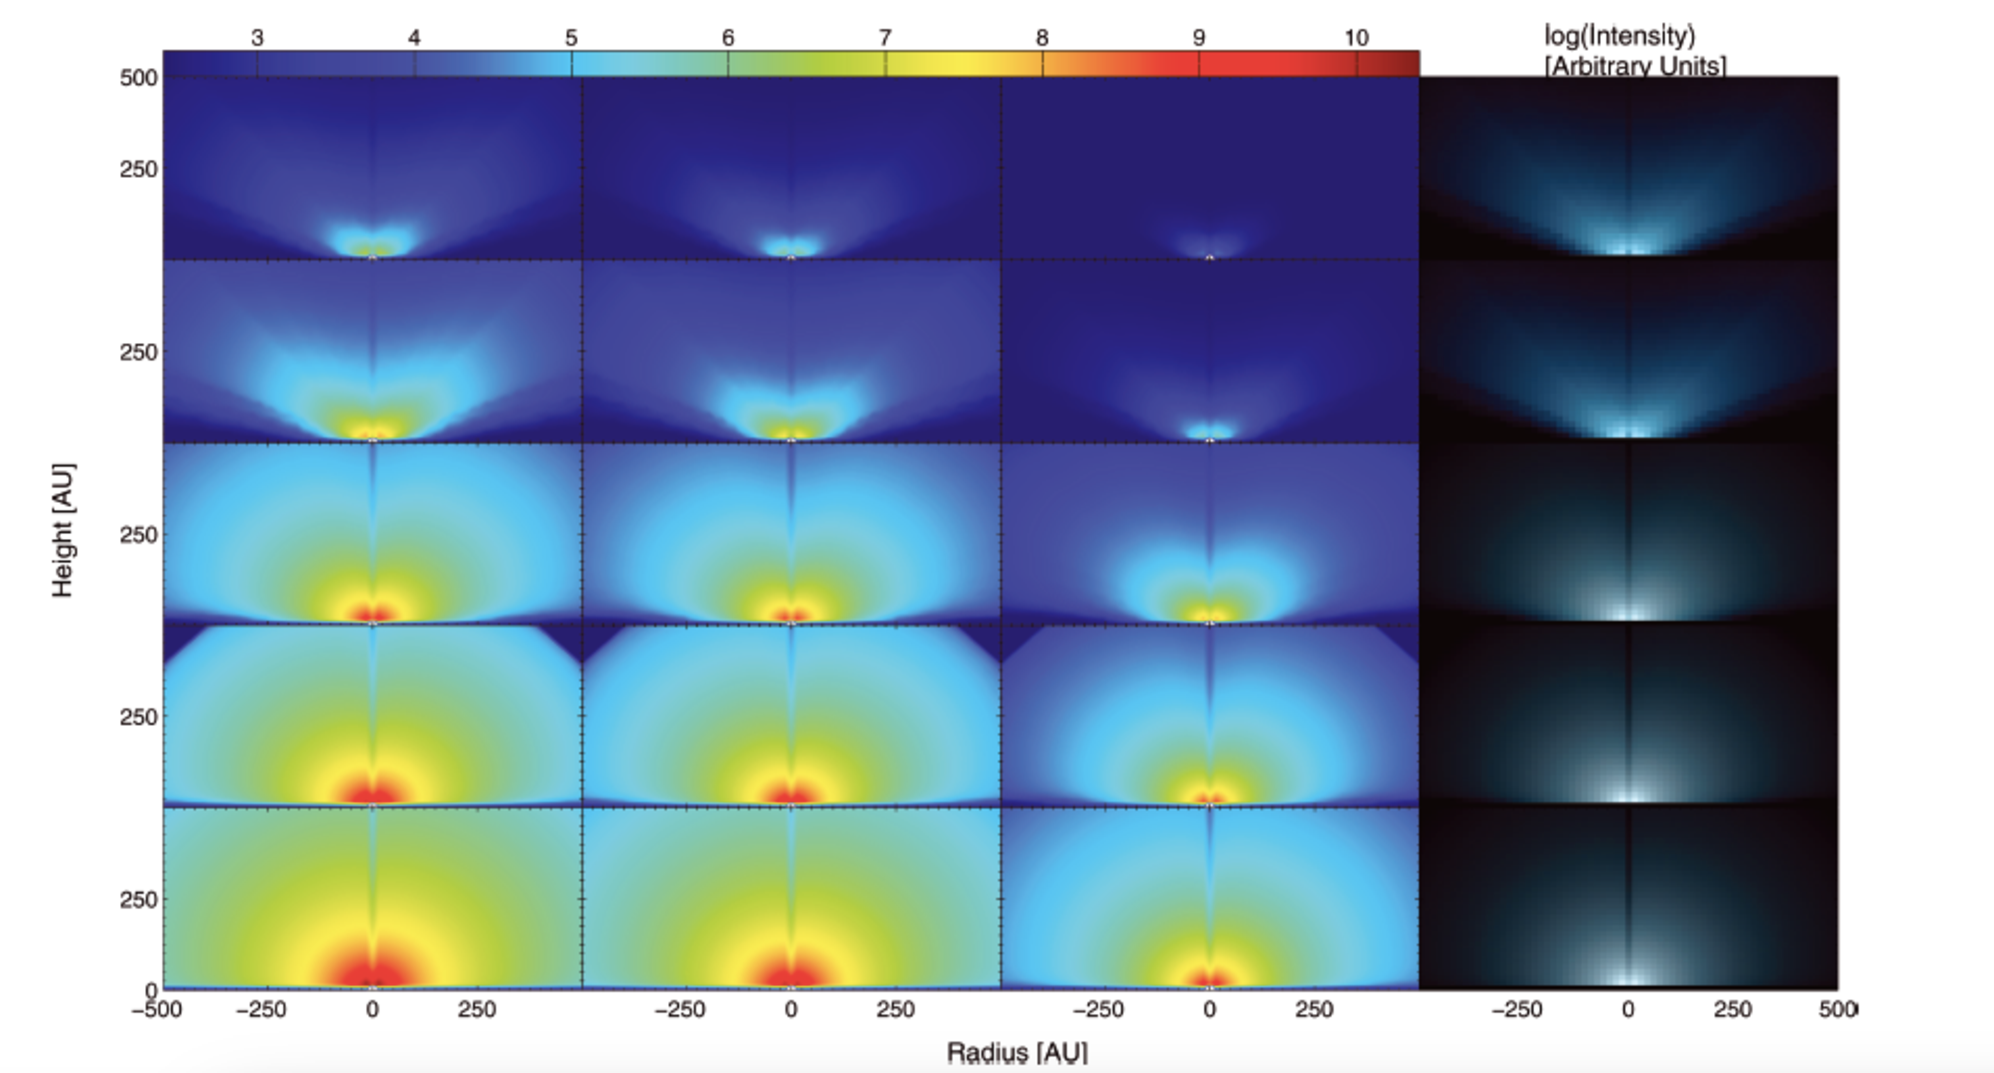
\includegraphics[width=0.95\textwidth]{wingnut.pdf}
  \caption{Image from Owen, Ercolano \& Clarke (2011b): Synthetic images for
    disc models with irradiating fluxes $\phi = 1e41.... 1e45 phot/sec$ ,
    the \caphighlight{far left-hand column} shows the image in the H band,
    the \caphighlight{next column} displays the K band and the
    \caphighlight{other next column} displays the L band. The
    \caphighlight{far right-hand column} displays an red giant branch
    composite image (L,K and H bands, respectively). The images are
    individually scaled so that there is a 5 dex spread between the
    brightest pixel and the darkest. All images assume that the disc is
    edge-on, therefore the stellar emission is blocked out by the presence
    of the optically thick disc.}
  \label{fig:maps}
\end{figure}

While the calculations of Owen, Ercolano \& Clarke show that indeed a
significant amount of small grains can be expected in photoevaporative
winds, they present however
some serious limitations that make them unsuitable for application to our Research
Unit tasks. 
First of all, these calculations are limited to the EUV-case only. The
X-ray photoevaporation case, which is likely dominant amongst T-Tauri
stars, is completely different and significantly more complex than the EUV case. 

Another important shortcoming of Owen, Ercolano \& Clarke (2011b) is
that they do not account for dust evolution in the underlying disc. An
MRN (Mathis, Rumpl, Nordsieck 1977) size distribution with standard gas-to-dust ratio of 100 is
assumed everywhere in the disc. The resulting dust density and size
distribution in the wind is thus necessarily incorrect. Given the
central role played by dust grains for the chemistry, our project will
couple dust evolution in the underlying disc to the wind entrainment
problem for the X-ray driven winds around T-Tauri stars.  

\subsubsection{Numerical approaches}

The dynamics of dust grains in protoplanetary discs can be studied
either by directly integrating the orbits of a large number of dust
'super-particles' (that sample the local properties of the dust
population) or by solving the collisionless Boltzmann equation for the
particle distribution function. For a population of very small
(tightly coupled with the gas) dust particles, the Boltzmann equation
can be reduced to the zero pressure fluid equation (Cuzzi et al.\ 1993,
Garaud et al.\ 2004). This 'two-fluid' approach has been used to study
planet-disc interactions (Paardekooper \& Mellema 2004, 2006; Zhu et
al.\ 2012). This is however limited to a single population of
small particles, it cannot account for the full velocity distribution
of the grains at a single location, and it is not able to capture
strong density gradients. The particle approach has the great
advantage to follow the evolution of solid particles with different
physical properties, perfectly recovering the dust dynamics in the
limit where the grains are decoupled from the gas (Youdin \& Johansen
2007; Miniati 2010; Bai \& Stone 2010). This method has also been
applied successfully to the study of planet disc interaction adopting
both SPH and grid-based codes (Fouchet et al.\ 2007, 2010; Ayliffe et
al.\ 2012; Lyra et al.\ 2009; Zhu et al.\ 2014). The grid codes are
preferred because they do not introduce a large artificial viscosity
that can affect the evolution of low-mass planets. Moreover, the
accuracy needed to properly model the evolution of the gas and dust
component in a protoplanetary discs is strongly dependent on the
choice of the grid geometry (Lyra et al.\ 2009; de Val-Borro et
al.\ 2007), requiring more computational effort in a cartesian grid
than in a cylindrical or spherical one. 

Dr.\ Picogna, who is currently employed as a postdoc in the group of PI
Ercolano, has implemented a population of dust
particles in the modern grid-based code PLUTO (Mignone et al.\ 2012)
that can evolve both in a cylindrical and spherical coordinate system
(Picogna, Stoll \& Kley, in prep.). This approach is thus ideal to
study the evolution of different dust particle populations in
protoplanetary discs. As detailed in the next section, this method,
coupled with the photoevaporation model implemented in PLUTO, will be
adopted to self-consistently model dust particles entrained into the
wind from the disc atmosphere for a number of selected cases.

The recent work of Hutchison et al.\ (2016a,b) used a new algorithm to
treat a wind in an SPH code. The wind is
treated using unequal-mass, one-fluid SPH. Using new techniques
developed by these authors they are able to simulate two-fluid dynamics
in highly stratified atmospheres. The work currently represents 
only a proof of concept, suggesting, however, that these novel
techniques may in 
the future be applied to study interesting aspects of gas and dust
dynamics in the wind. At present, however, the models are very
idealised, approximating discs and winds by a thin, non-rotating,
plane-parallel atmosphere.  This technique is thus not yet mature to
be used for the purposes of our project.

\subsection{Grain sizes and abundances at the base of the wind}

One key element of this project is to investigate the impact of the
underlying grain population on the observability of photoevaporative
winds. To this end we will use the state of the art coagulation code
from \citet{2010A&A...513A..79B} which solves for the evolution of the
particle distribution due to coagulation, fragmentation, and erosion,
as well as radial transport by drift, mixing, and gas advection. The
resulting particle size distribution $\Sigma_\mathrm{d}(t,r,a)$ is
then a function of distance to the star $r$, particle size $a$, and
time $t$. Treating the growth in a vertically averaged way (i.e.
using surface densities instead of volume densities) is generally a
good approximation since vertical settling and mixing time scales are
short for growing particles. However, for this project, the vertical
distribution of particle sizes is important as it determines the sizes
and abundances of particles at the base of the photoevaporative flow.

At the beginning of the project, we will use vertical distributions of
particles that are in a steady state between mixing and settling, such
as derived by \citet{2009A&A...496..597F}. These are simple analytical
equations, which need to be numerically integrated for each particle
size. This technique is already available and has been used for
calculating the observational appearance of simulated disks e.g.
in \citet{2015ApJ...813L..14B} and many other works. This should give
a good first representation of the particles that are present at the
base of the flow.

At a later point, these prescriptions can be updated with a more
sophisticated treatment of coagulation and transport processes: at
high dust-to-gas ratios small grains can be ``trapped'' closer to the
mid-plane due to frequent collisions with other particles
\citep{2016ApJ...822..111K}. When photoevaporation has preferentially
depleted the gas, thus raising the dust-to-gas ratio in the disk, this
effect could potentially affect the amount of small dust grains that
are mixed up to the base of the photoevaporative flow. The results of
\citet{2016ApJ...822..111K} can be used to estimate this effect.
Some time during the second  year of this project, we expect the ERC
group of T.\ Birnstiel to have a working 2D dust coagulation and
transport model which will allow us to check for differences between
the earlier approaches (steady state distributions) and models that
take the time evolution and collisional processes into account.

\subsection{Project-related publications}

% Please list your own publications related to the proposed project, 
% adhering to the rules of the DFG guidelines 1.91. In brief, please note: 
% - Up to 10 publications
% - The work must be published or accepted.
% - Publications on astro-ph (arXive, SPIRES or articles with a DOI) count as published. 
% - Any work that is only in the status ``accepted'' MUST be attached to the proposal
%    together with the acceptance letter.
% - All publications in this section CAN be attached to the proposal. Please limit these
%    attachments to a minimum and please note that the reviewers may not read the attachments -
%    the proposal has to speak for itself.
% - The number of allowed publications refers to the sum of the publications listed
%    in ``1.1.1 Articles published or officially accepted by publication outlets...'' and 
%    in ``1.1.2 Other publications''. Publications which only exist on public repositories 
%    belong into the category ``Other Publications''.

%\subsubsection{
%Articles published or officially accepted by publication outlets with scientific quality assurance;
%book publications}

\begin{literature}
\item {\bf Birnstiel, T.}; Dullemond, C.P. \& Brauer, F.: \textit{Gas and
dust evolution in protoplanetary disks}, 2010, A\&A 513, 79. In this paper we
  present the basic code for the evolution of the disk and the dust. The
  latter follows the dust coagulation, fragmentation, settling and radial
  drift of the dust.
\item{\bf Birnstiel, T.}; Klahr, H. \& {\bf Ercolano, B.}: \textit{A simple model
for the evolution of the dust population in protoplanetary disks}, 
  2012, A\&A 539, 148. In this model the flow of pebbles from the outer
  disk regions into the inner planet forming disk regions is studied,
  and an easy to use model derived.
\item {\bf Birnstiel, T.}; Andrews, S.; Pinilla, P. \& Kama, M.:
\textit{Dust Evolution Can Produce Scattered Light Gaps in Protoplanetary Disks},
2015, ApJL 813, L14. Here we applied the vertical steady state
settling mixing distribution to calculate the observational appearance
of simulated disks.
\item {\bf Ercolano, B.}; Drake, J.; Raymond, J. C.; Clarke, C. C.:
\textit{X-Ray-Irradiated Protoplanetary Disk Atmospheres. I. Predicted Emission-Line Spectrum and Photoevaporation},
2008, ApJ 688, 398. We present mocassin two-dimensional
photoionization and dust radiative transfer models of a prototypical T
Tauri disk irradiated by X-rays from the young pre-main-sequence
star. In this work a first estimate of X-ray photoevaporation rates is
given, hinting at the relevance of this process for disc dispersal
\item {\bf Ercolano, B.}; Clarke, C. C.: Drake, J.;
\textit{X-Ray Irradiated Protoplanetary Disk Atmospheres. II. Predictions from Models in Hydrostatic Equilibrium},
2009, ApJ 699, 1639. In this follow-up paper we take into account the
response of the disc structure to the X-ray heating and demonstrate
that even in this case the X-ray photoevaporation rates remain
substantial. A hydrostatic solution is reached iteratively with the
full photoionisation problem. 
\item Owen, J. E.; {\bf Ercolano, B.}; Clarke, C. J.; Alexander, R. D.
\textit{Radiation-hydrodynamic models of X-ray and EUV photoevaporating protoplanetary discs},
2010, MNRAS, 401, 1415. Starting from the hydrostatic solutions of
Ercolano et al 2009, we perform the first radiation-hydrodynamic
solution of an X-ray irradiated disc. Robust mass-loss-rates and
profiles are calculated for this model, suggesting that X-ray drive
the dispersal of discs. 
\item Owen J., \textbf{Ercolano B.}, Clarke C.  \textit{
  Protoplanetary disc evolution and dispersal: the implications of X-ray photoevaporation}, 2011a, MNRAS, 412, 13.
  We explore the role of X-ray photoevaporation in the evolution and
  dispersal of viscously evolving T Tauri discs. Our models confirm
  that X-rays play a dominant role in the evolution and dispersal of
  protoplanetary discs giving rise to the observed diverse population
  of transition discs, including some of those with massive outer
  discs, some of those
  with gas in their inner holes and some of those with detectable accretion
  signatures.  
\item Owen J., \textbf{Ercolano B.}, Clarke C.  \textit{
    The imprint of photoevaporation on edge-on discs}, 2011b, MNRAS, 411, 4103.
  We perform hydrodynamic and radiative transfer calculations of a
  photoevaporating disc around a Herbig Ae/Be star to determine the
  evolution and observational impact of dust entrained in the wind. We
  find that the wind selectively entrains grains of different sizes at
  different radii resulting in a dust population that varies spatially
  and increases with height above the midplane.
\item Owen J., Clarke \& \textbf{Ercolano B.}  \textit{On the theory of disc photoevaporation}
  2012, MNRAS, 422, 1880. We derive analytical scaling relations and
  derive estimates for the total mass-loss rates, as well as
  discussing the existence of similarity solutions for flows from
  primordial and transition discs. In this paper we catch a first
  glimpse at a new process for the clearing of the very last stages,
  which we name ``thermal sweeping''.
\item \textbf{Ercolano B.}, Owen J.  {\em Blueshifted [O I] lines from
    protoplanetary discs: the smoking gun of X-ray photoevaporation},
  2016, MNRAS 460. 3472
  We produce new synthetic observations of a particularly promising
  diagnostic, and demonstrate that the observations available at the
  time (before Simon et al.\ 2016) are consistent with the
  photoevaporation model. We show however that this line cannot be
  used to measure mass-loss-rates. 
\end{literature}


%\subsubsection{Other publications}
%
%None
%
%\subsubsection{Patents}
%
%None
%
%\paragraph{Pending}
%
%None
%
%\paragraph{Issued}
%
%None

\section{Objectives and work programme}
\renewcommand{\leftmark}{\sc Objectives and work programme}

\subsection{Anticipated total duration of the project}

36 months

\subsection{Objectives}
In this project
we aim to determine the dust content and size distribution of photoevaporative winds for a range of stellar, disc and wind parameters,
using realistic descriptions for grain evolution in the underlying
disc. 

This will allow us to : 
\begin{enumerate}
\item Build a dust model for photoevaporative winds to be used in
astrochemistry and radiative transfer calculations.
\item Estimate the observability and observation characteristics of
the dust phase in photoevaporative winds.
\end{enumerate}

\subsection{Work programme including proposed research methods}
% for each applicant

\connect{In this project we will first use the semi-analytical approach described in
\cref{sec:analytical-approach} coupled to models for the
evolution of dust grains in the disc in order to efficiently produce
dust entrainment models for the complete set of X-ray photoevaporation
wind solutions calculated in project B1. The dust models will then be
passed on to project B2 (chemical models), incrementally as they are
calculated.}

There are several reasons for choosing the semi-analytical approach
over fully numerical approaches (SPH or grid-based). First of all,
semi-analytical 
approaches are much more efficient for our aims. We will make
use snapshots from the hydrodynamical calculations, since, to first
order, the grain entrainment problem can be decoupled from the photoevaporation 
problem. Indeed 
dust grains entrained in the wind do now provide tangible extinction
at X-ray frequencies, hence the wind structure and rate are
not sensitive to the dust distribution in the wind. The dust
entrainment calculation can thus be performed by
post-processing snapshots of the radiation-hydrodynamic calculations,
allowing us
to use the same wind solution and changing (e.g.) the underlying dust
distribution in the disc, according to different models and
prescriptions. 

It is perhaps worth mentioning that the dust evolution in the
underlying disc is however strongly coupled to the evolution of the gas
in the disc. A full radiation-hydrodynamic simulation of the gas and
dust which also simultaneously solves the dust coagulation and drift
is however beyond what is currently feasible. It is however possible
to perform a gas radiation hydrodynamics calculation which includes
dust particles, not accounting for coagulation (e.g.\ Picogna, Stoll \&
Kley ,
in preparation). If time allows, we will perform a number of such
(expensive) calculations to compare with the semi-analytical
ones. This is particularly important for transition disc models, where
the dust may be pushed back away from the inner edge of the disc due
to the pressure gradients in the gas, thus resulting in a  lower dust
content in TD winds, compared to full discs.  In any case, a more
comprehensive set of these simulations will be performed during the
second funding period of the Research Unit.  


The work proposed here will be carried out by a PhD student supervised by
Prof.\ Ercolano (LMU) with the help of Dr.\ Birnstiel (LMU), who will
advice, respectively, on the dust entrainment calculations and the 
coupling with the dust evolution models for the underlying disc. 

\subsubsection{Research Tools and Inputs}

For this project we will need the following tools:
\begin{enumerate}
\item Photoevaporative wind solutions for EUV-driven
models for T-Tauri and Herbig stars. These are easily computable 
using the models that are described in the literature \citep[e.g.,][]{2004ApJ...607..890F}.
\item \connect{Photoevaporative wind solutions for X-ray photoevaporated
models. These will be provided from project B1.}
\item One-dimensional dust growth models. These codes are published
and available within the group: simulation code of 
 \citet{2010A&A...513A..79B} and the parameterized model of
 \citet{2012A&A...539A.148B}. The one dimensional results will be
 coupled to prescriptions of vertical mixing \citep[e.g.]{2009A&A...496..597F}
\item Two-dimensional dust evolution results/parameterisation from the
  ERC-funded projects of Dr.\ Birnstiel.
\item A 3D radiative transfer code to post-postprocess the wind
models with the calculated grain populations. For this we can use the
streamlined version of the {\sc MOCASSIN} code developed by the PI
(see description below) and/or use  of the
RadMC3D code developed and maintained by Prof.\ Dullemond. 
\end{enumerate}

\subsubsection{Research Plan} 

The project will proceed in stages of increasing complexity. We will start
by setting up a framework that can be benchmarked against available
calculations and progressively adding new elements, as they become
available from other projects. The plan has been designed to fit a
PhD student, who will have the opportunity to develop a new theoretical
model as well as acquainting her/himself with standard numerical
techniques (e.g.\ radiation-hydrodynamics, dust evolution models,
radiative transfer). 

\connect{The most important science product from this project is the set of
grain models developed for the  X-ray driven wind. These are needed by
project B2 for the chemical calculations, as the dust
grains dominating the opacities in the FUV are not equally distributed
in the wind (see e.g.\ Owen, Ercolano \& Clarke, 2011b, Hutchison et
al.\ 2016ab) and they thus affect the chemistry in the wind
differently in different parts.}

\paragraph{Preparatory Work}


\begin{figure}
  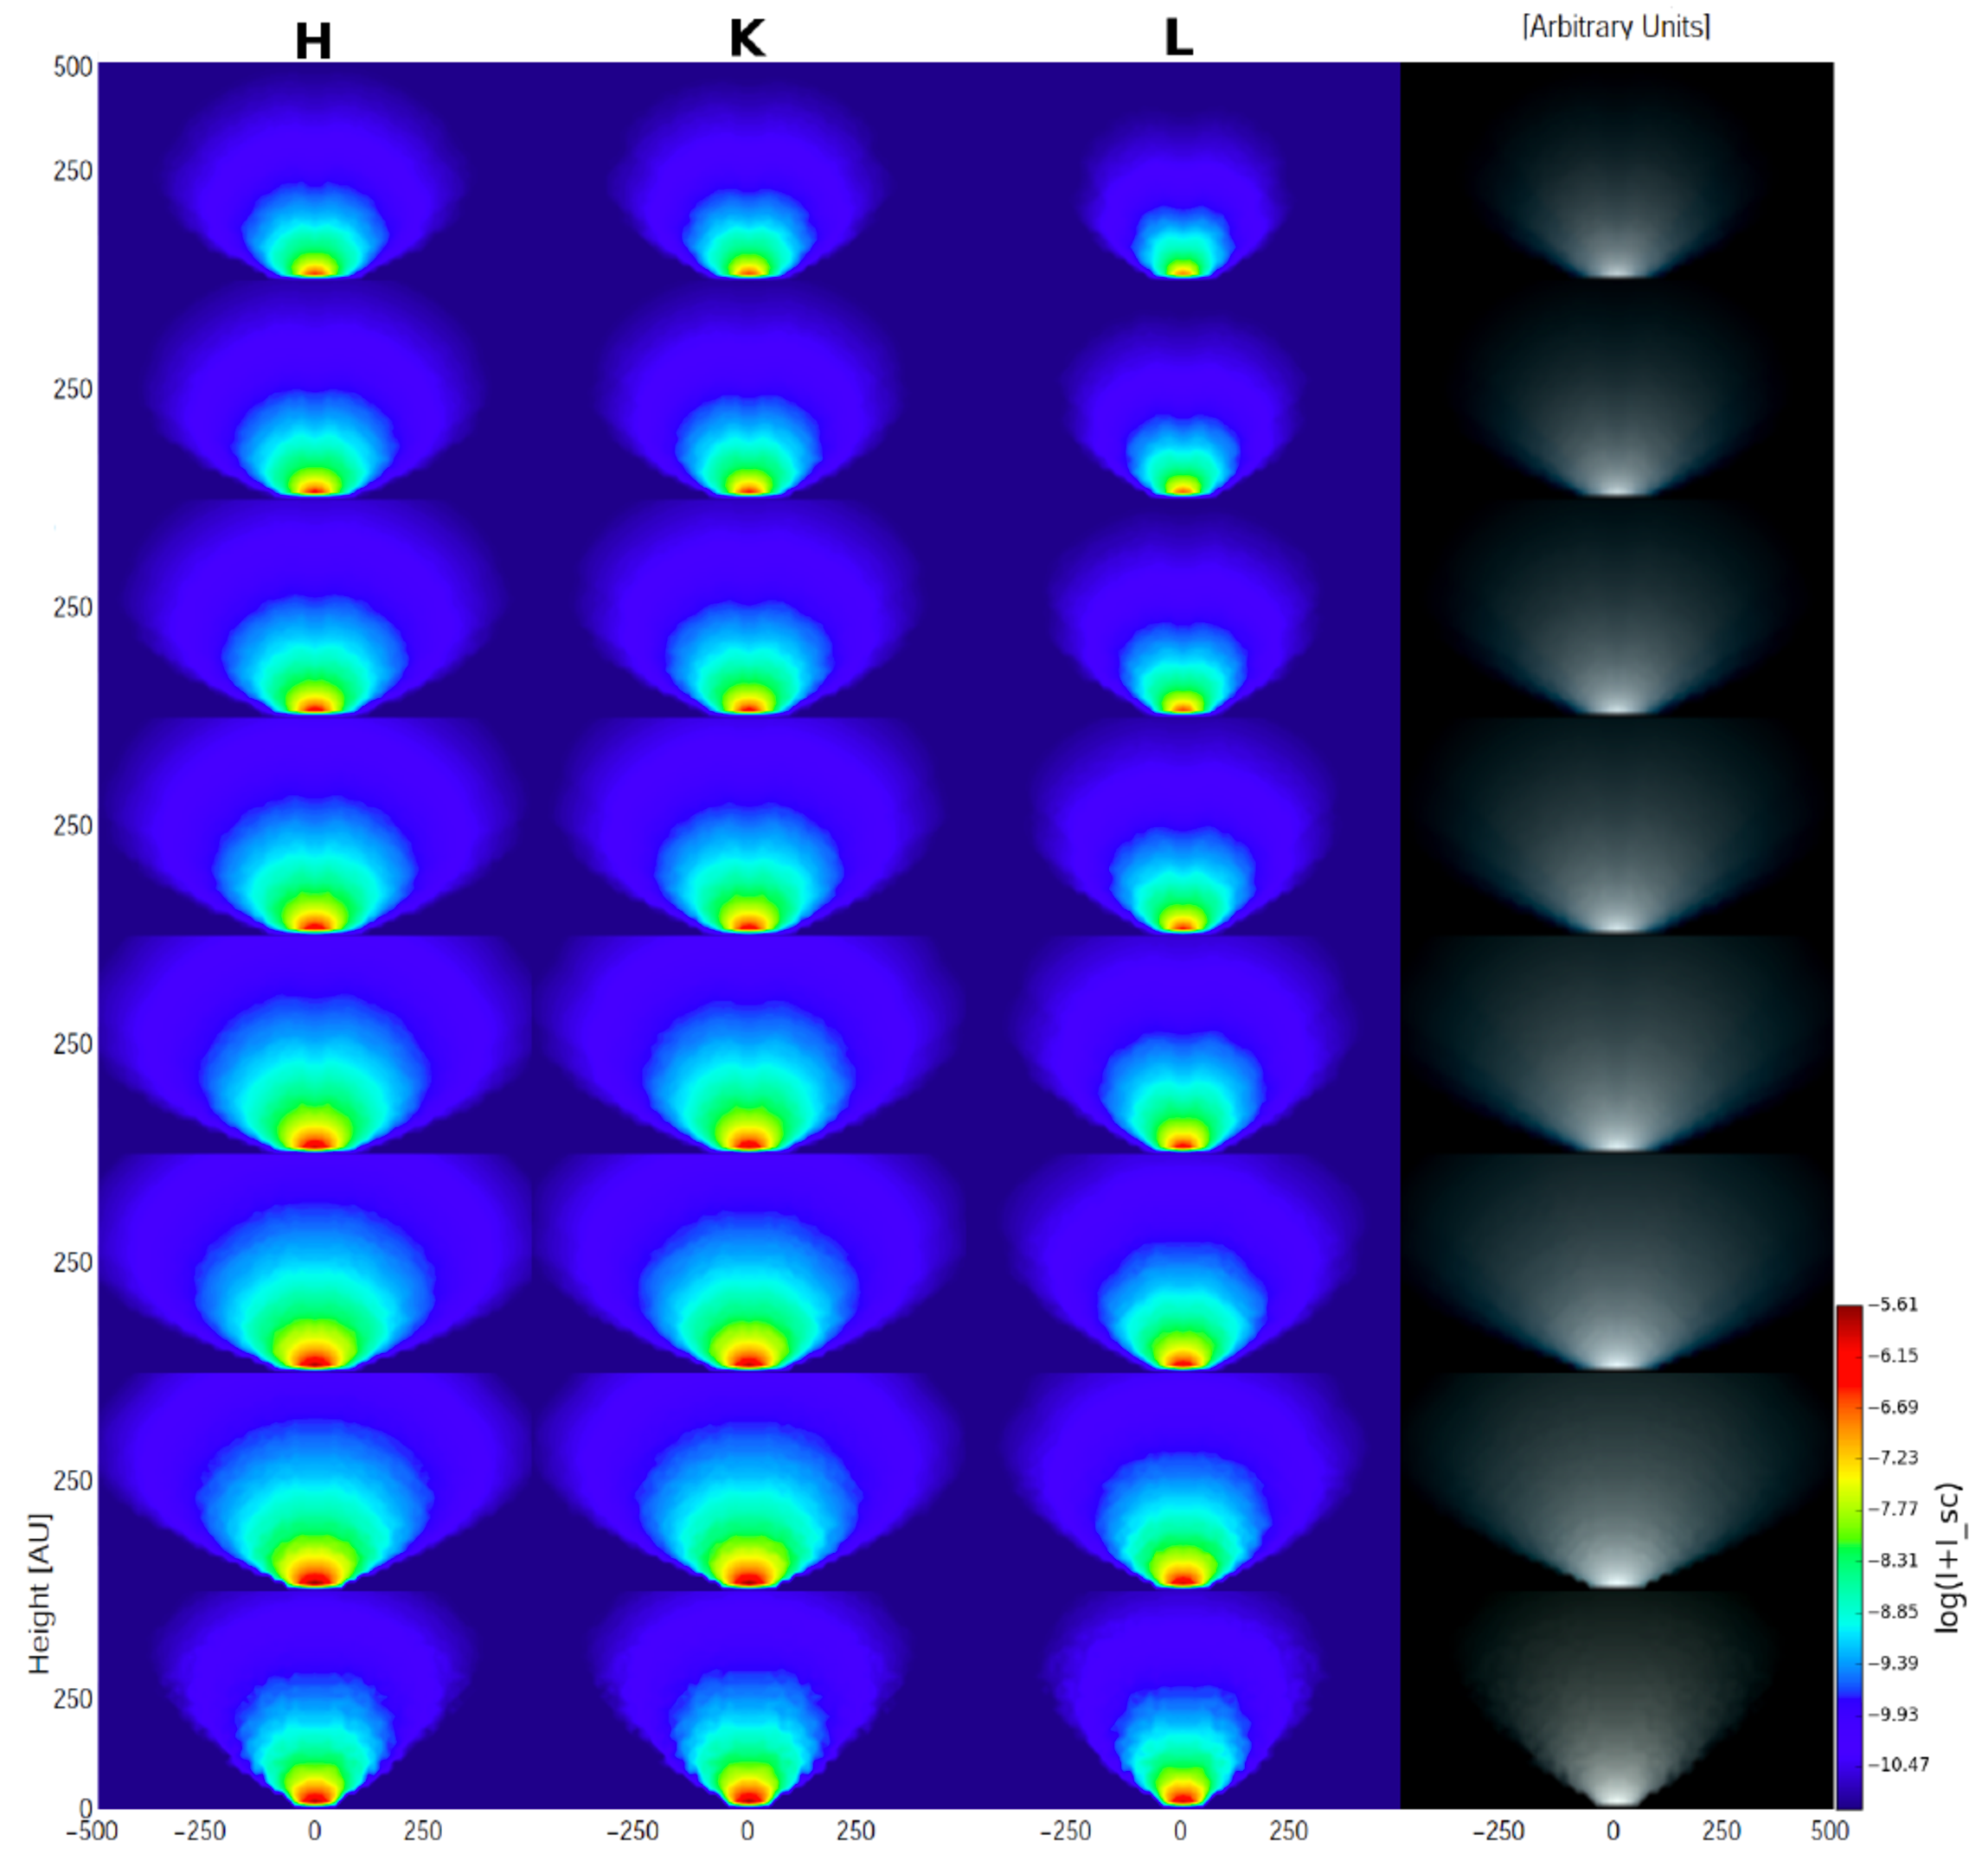
\includegraphics[width=0.95\textwidth]{mrntruncation.pdf}
  \caption{Effect of sequential truncation of MRN on the
    image. \caphighlight{Columns, from left to right respectivley:} H: (1.5
    - 1.8)$\mu$m, K: (2 - 2.4)$\mu$m, L: (3 - 4)$\mu$m.  Rows from top to
    bottom correspond to MRN in the disk with respectively: a$_{min}$ = 5,
    10, 20, 42.4, 86, 170, 360, 730 nm and a$_{max}$ =
    1mm. \caphighlight{First three columns of all rows} are normalized such
    that there are 5 dex between the brightest value in the L band of all
    images, representing the white pixel and the black pixel. Figure taken
    from the LMU Master Thesis of Denis Mehmedov, 2015.}
  \label{fig:densitygrowth}
\end{figure}


\begin{figure}
  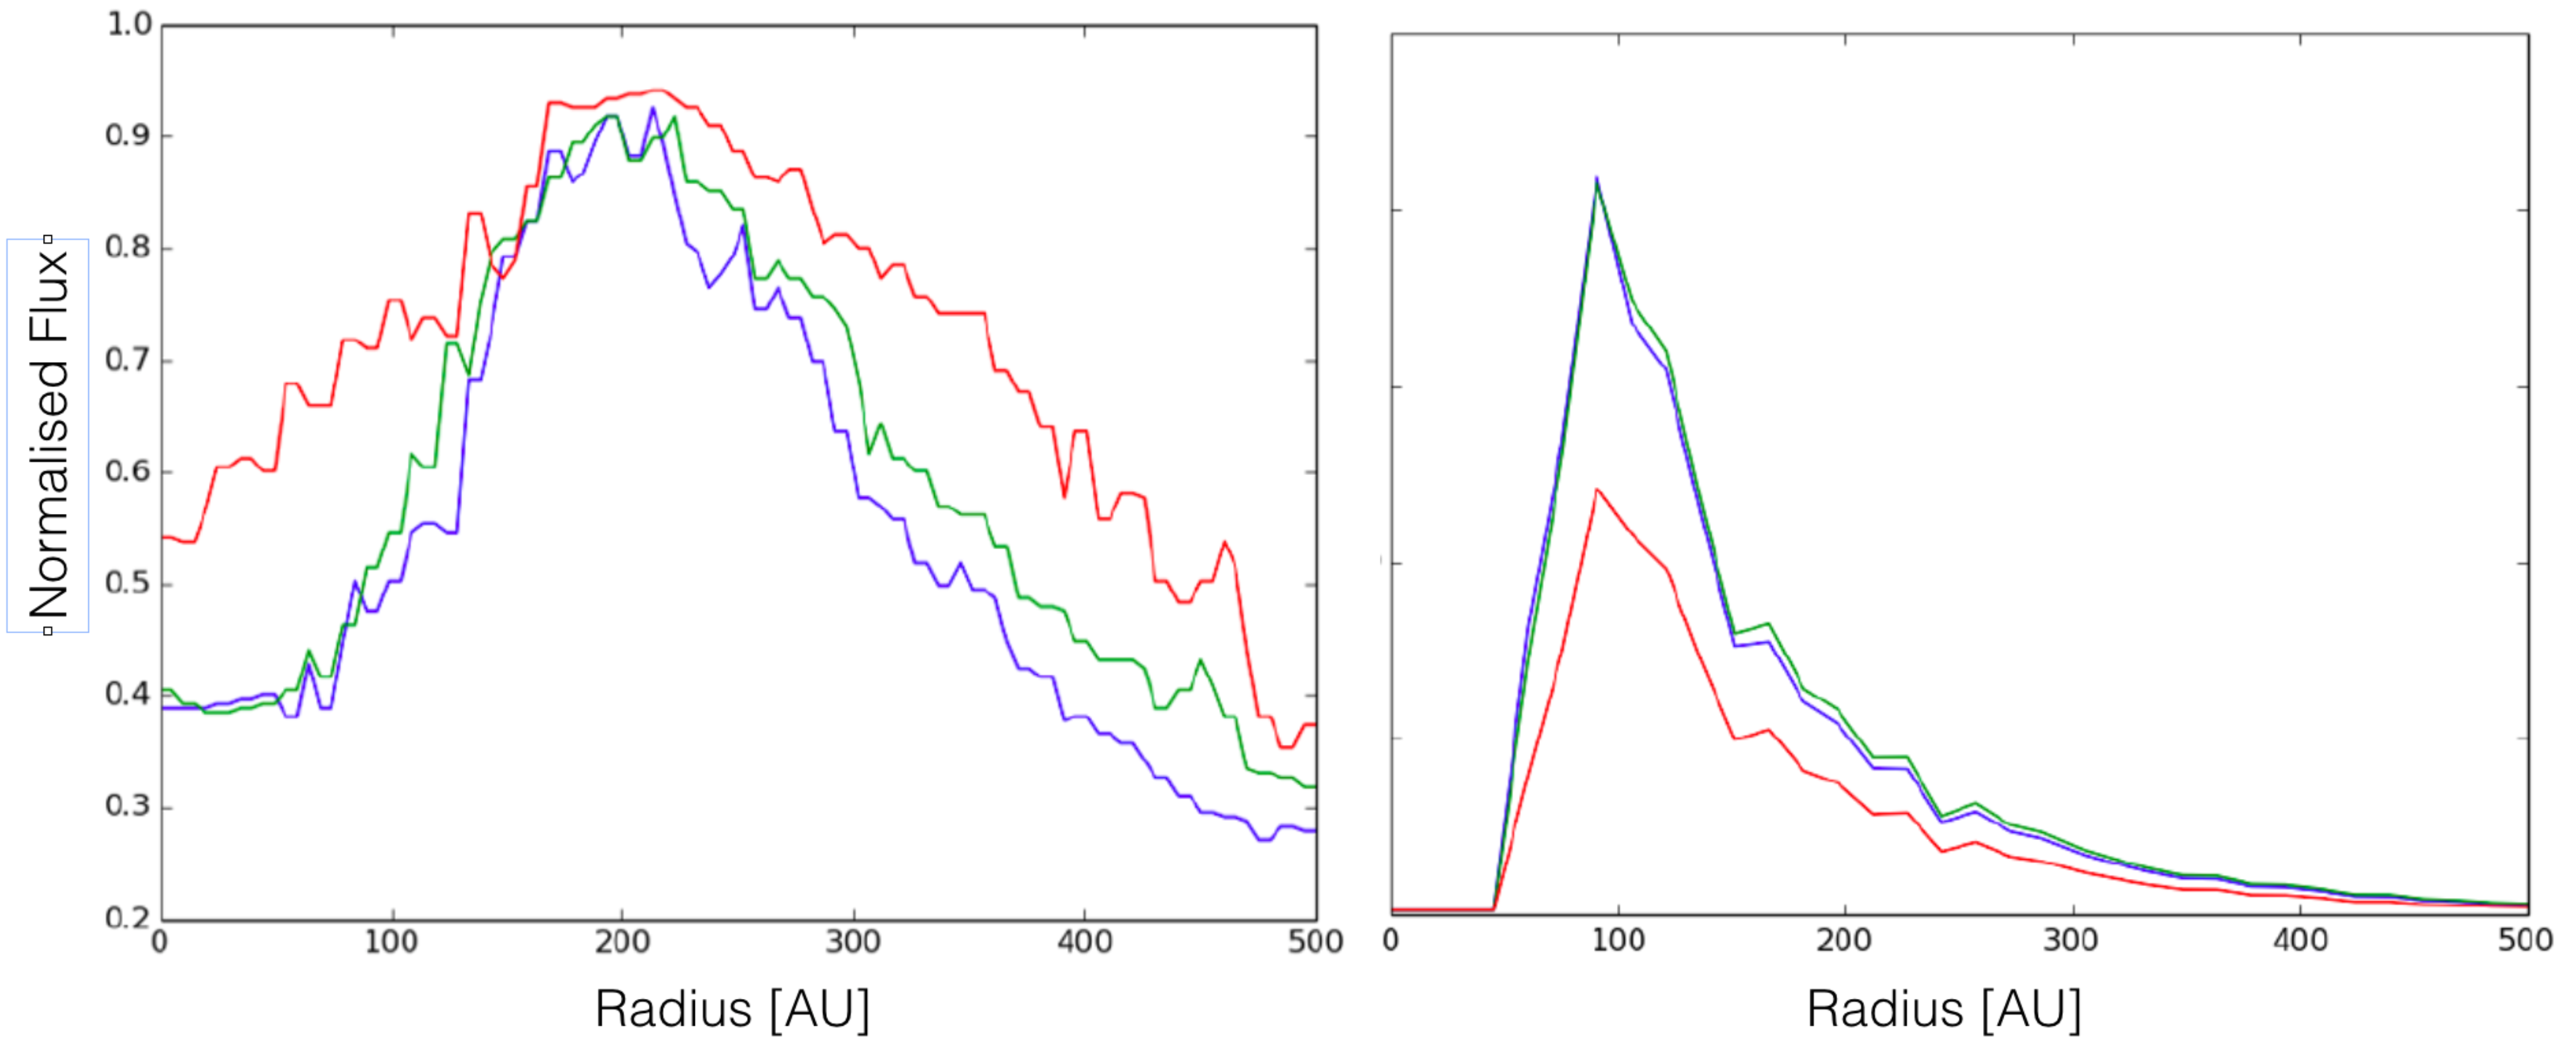
\includegraphics[width=0.95\textwidth]{colorinversion.pdf}
  \caption{\caphighlight{Left Panel:} Color plot of the slice at 100AU in
    the observational images extracted from Perrin and Graham
    (2006). \caphighlight{Right Panel:} The same for out simulation with the
    maximum truncation of the MRN ($a_{min}$=730nm). Figure taken from the
    LMU Master Thesis of Denis Mehmedov, 2015. }
  \label{fig:colourgrowth}
\end{figure}


The methodology described in Owen, Ercolano \& Clarke (2011b), has been
used in the group of the PI Ercolano to develop a suit of codes which
take the gas density and velocity of the EUV-only wind and the stellar
irradiation spectrum as an input and calculate the dust density and
size distribution in the wind. 

The resulting codes are the product of first a bachelor and then a master
student project in the group of PI Ercolano. The aim of the bachelor project
performed by George Dadunashvilli in 2013 and of the master project
performed  by Denis Mehmedov in 2014, was to asses the role played by
dust growth in the underlying disc on the appearance of the wind in
the case of the EUV-only driven wind from the Herbig star studied by
Owen, Ercolano \& Clarke (2011b). 

The projects were motivated by the failure of the Owen, Ercolano \&
Clarke (2011b) models in reproducing the colour gradient in the observations
of  PDS 144N (Perrin et al.\ 2006), which show redder emission at
larger heights above the disc. 

The main results of the two projects can be briefly summarised as follows. 
In the case of an EUV-only wind, the removal of small grains from the disc atmosphere due to grain
growth produces an overall reduction in the total dust density in the
wind. This can be seen in Figure~\ref{fig:densitygrowth}, where the
dust density distribution in the wind is compared for the case of an
underlying disc grain size distribution following a 
standard MRN (Mathis, Rumpl \& Nordseick 1977) and for a truncated 
MRN. The colours of the wind are also affected by the removal of small
grains in the disc, but not enough to reproduce the observations. A
comparison of different calculations for different grain size cut-offs
are shown in Figure~\ref{fig:colourgrowth}. 

There are a number of problems with these preliminary results
however. First of all
a full exploration of the parameter space, even if only for the
EUV-only case is beyond the scope of bachelor or even master
projects. This is one of the reason why these results have yet to be 
published. Furthermore an unrealistically simplified approach to the 
including the effects of grain growth was used. Simply a cut-off was
applied to the minimum grain size in the MRN distribution of the
underlying disc. This led to the fact that we have been limited to a
maximum cut-off of 0.73$mu$m. A cut-off at larger sizes would have led
to a virtually dust-free wind. This is unrealistic since the growth of
grains in a more realistic coagulation model leads to a larger population (by
number) of a few micron-size grains compared to a standard MRN which
is truncated at say 1$mu$. 

 Nevertheless, the legacy of these projects is a suite of
codes, which were compared in detail, and result now much improved
compared to the Owen, Clarke \& Ercolano (2011b) tools. These can be
used as a starting point and upgraded by the PhD student employed for the project.  


\paragraph{Months 1-12}

The student will start by producing wind solution for the EUV case
from the work of \citet{2004ApJ...607..890F}, which may be applicable
to Herbig stars. For that she will use the standard version of the
PLUTO code (Mignone et al.\ 2007, 2012) in
two-dimensional mode. Note that no additional column density/Stroemgren radius
calculations need to be used in order to implement the Font et
al.\ (2004) solutions for EUV winds. This solution simply treats the
wind as an isothermal gas with sound speed, $c_s =
\SI{10}{km.s^{-1}}$.
The number density at the base of the wind is also fixed and is a simple
function of radius, mass of the central star, gas sound speed and
ionising stellar flux (Font et al.\ 2008, Alexander 2009, Hollenbach et
al.\ 2004). We will be able to validate our solutions with those in the
literature, which is an important step, particularly in a project led
by a PhD student. 

The student will then proceed to calculate the dust
distribution in the wind, under simplifying assumptions for the
underlying dust distribution in the disc as in \citet{2011MNRAS.411.1104O}. In
brief, streamlines from the base of the flow to the edge of the grid
will be computed and along each of them, the force balance between the
drag force, gravity and the centrifugal force will be calculated. A
positive net force on a grain along the streamline will indicate that
the grain is entrained.

Once dust abundance and size distributions have been obtained for the
wind, radiative transfer calculations will be performed to produce
synthetic continuum observations at several disc inclinations. 
These first models will be benchmarked against the solutions
of \citet{2011MNRAS.411.1104O}. Note that we have produced a
streamlined version of our MOCASSIN code which we used to produce the
images in \citet{2011MNRAS.411.1104O}, as well as in the subsequent
bachelor and master thesis projects. However the RADMC-3D code
developed by Prof.\ Dullemond (co-speaker to the Research Unit) is also
available to us for comparison. 

After the benchmarking tests, we will be sure that we have developed a
solid framework which can now be applied, for the
first time, to the calculation of the dust component entrained in an
X-ray driven photoevaporative wind. The wind solutions of Owen et
al.\ (2010, 2011, 2012) and Ercolano \& Owen (2016) are readily
available and they could provide a starting point, \connect{until new 
wind solutions become available form project B1.} This may however
not be necessary as the new wind models for the X-ray case
are already being calculated by Dr.\ Picogna, who is employed to do the
preparatory work for project B1. It is therefore likely that an
initial set of high resolutions new X-ray wind solution may already be
available to the student right from the start of project C2.
 
\connect{As the first dust models for the X-ray driven wind become available
they will be immediately passed on to project B2 (Astrochemistry), for
inclusion in the chemical models to be then updated when the new
models including dust evolution in the disc become available (see next
section).} 

We will perform new radiative transfer calculations of the dusty
X-ray driven wind to produce synthetic continuum observations and
provide a first estimate of the observability of such winds with
current/future instrumentations. Our results may motivate
observational campaigns led by collaborators (e.g.\ the group of
Prof.\ Henning), the outcome of which, however does not influence the
success of the research aims of our projects. In
Figure~\ref{fig:dustywind} we show an example of a possible outcome of
our models. The image shows \todo{???????}

\todo{The figure reference fig:dustywind is not defined.}

\paragraph{Months 13-24}
 
At this point we will be in a position to significantly improve on
this work by considering more realistic grain abundances and size
distributions for the underlying disc. 

We will first couple the grain entrainment calculations to simple
prescriptions of dust  evolution \citep[e.g.,][]{2012A&A...539A.148B}
obtained from the one-dimensional models of
\citet{2010A&A...513A..79B}. The one dimensional models describe the
evolution of dust that is mostly in the mid-plane, i.e.\ well below the
base of the wind, where the grains may be entrained from. The
Birstiel, Klahr \& Ercolano (2012) prescriptions will then need to be
coupled to vertical mixing prescriptions \citep{2009A&A...496..597F} in order to
estimate the grain distributions at the wind-launching location,
obtained from the hydro simulations. 

Complementary to this project the ERC-funded team led by
Dr.\ Birnstiel aims to develop new two-dimensional (both
radius-height and radius-azimuth) dust evolution
models. When these new models become available, the student will work
closely with Dr.\ Birnstiel to include elements of these new results
in our calculations. 

\paragraph{Months 25-36}

In this last year of the first funding period the whole machinery will
be in place. We will now be able apply it to a wide parameter
space of disc winds, \connect{producing sets of dust models to be passed on to
project B2 for the chemical calculations.}

We will also perform comprehensive radiative transfer calculations of
the obtained structures to compare with available observations or to
make more detailed observability predictions, which may further guide
future observing proposals. We will join forces with expert
collaborators on scattered light observations (e.g.\ Prof.\ Henning,
Prof.\ Dullemond) to
plan new proposals, however we stress that failure to obtain new
observations as well as eventual non-detections do not preclude the
main aim of this project to be achieved, i.e.\ the development
of dust models and dust distributions in photoevaporative winds. 

If time allows, the student will collaborate with Dr Picogna (postdoc
in the group of the PI
Ercolano) to
produce full hydrodynamical simulations of disc winds, where the dust
component in the disc and wind is treated as particles (e.g.\ Picogna
\& Kley 2016). These calculations, which are computationally very expensive
will be useful as a piecewise comparison to the simpler methods previously
developed by the student in the project.  

Furthermore, as detailed in a previous section, we plan compare and contrast
the efficiency of dust entrainment for discs at different evolutionary
stages. A more comprehensive set of simulations, which may also include
photoevaporating discs with gaps opened by giant planets
(e.g.\ Rosotti, Ercolano et al.\ 2013, 2015), is expected to be
performed in the second funding period. 

\vspace{0.5em}


\subsection{Data handling}

The model data-grids will be made available on the Research Unit
dedicated server for use within the team. Furthermore we will provide
a set of diagnostic models to guide observers in the wider community,
which will be placed 
on the public partition of the server.
This public data will include sets containing the full size
distribution at every 2D point, as well as sets of the
mean/minimum/maximum grain sizes (the mean averaged in different
ways), as well as synthesised images in different bands which can be
directly compared to observations. 

\subsection{Other information}
% Please use this section for any additional information you feel is
% relevant which has not been provided elsewhere.

Not Relevant

\subsection{Information on scientific and financial involvement of international cooperation partners}

Not Relevant

\section{Bibliography}

\todo{Kees to Barbara: Shall I convert all your references to bibtex for
  you? Then we get a same style in all projects and it will be easier to
  handle.}

\begingroup
\renewcommand{\section}[2]{}%
\bibliographystyle{aa}
\bibliography{bibliography}
\endgroup

\section{Requested modules/funds}
\renewcommand{\leftmark}{\sc  Requested modules/funds}
% Explain each item for each applicant (stating last name, first name).

\subsection{Basic Module}

\subsubsection{Funding for Staff}
% Please note that funds for your own temporary position (“Eigene Stelleâ€)
% are not to be included here; this belongs to the separate “Module Temporary Positionâ€.

We require funding for one PhD student to be supervised at the LMU
by Prof.\ Ercolano.

\subsubsection{Direct Project Costs}

\paragraph{Equipment up to EUR 10,000, Software and Consumables}

Will be provided by the host institution. 

\paragraph{Travel Expenses}

Total: 9900 \EUR{}

Justification: Each year one national trip (e.g., meeting of
Astronomical Society, national meetings) and one international trip
(conference, visit to collaborators). During the course of the PhD 2
one week long visits to our main international collaborator, Dr J.
Owen (currently at Princeton University, will move to Imperial College
London in 2017).

Cost estimate: 
\begin{itemize}
\item National trip: 5 overnight stays, train/airfare,
conference fee; 1000 \EUR{} (3000 over 3 years).
\item International trip: 6 overnight stays, airfare, conference fee;
  1500 \EUR{} (4500 over 3 years).
\item Visit to/from J. Owen: airfare, 6 overnight stay 1200 \EUR{} (2400
  for 2 visits)
\end{itemize}


\paragraph{Visiting Researchers (excluding Mercator Fellows)}

Not Relevant

\paragraph{Other Costs}

None

\paragraph{Project-related publication expenses}

We request 750 \EUR{}/year (total 2250 \EUR{}) for publication expenses.

\subsubsection{Instrumentation}

None

\paragraph{Equipment exceeding EUR 10,000} 

None

\paragraph{Major Instrumentation exceeding EUR 100,000} 

None 

% \subsection{Module Temporary Position}
% 
% Not Relevant 
% 
% \subsection{Module Replacement Funding}
% 
% Not Relevant 
% 
% \subsection{Module Mercator Fellows}
% 
% Not Relevant 
% 
% \subsection{Module Public Relations Funding}
% 
% Not Relevant 

\section{Project requirements}
\renewcommand{\leftmark}{\sc Project requirements}

\subsection{Employment status information}
% For each applicant, state the last name, first name, and employment
% status (including duration of contract and funding body, if on a
% fixed-term contract).

Barbara Ercolano, Professor at the Ludwig-Maximilians-Universit\"at
M\"unchen  (permanent)



\subsection{First-time proposal data}
% Only if applicable: Last name, first name of first-time applicant.

Not Relevant

\subsection{Composition of the project group}
% List only those individuals who will work on the project but will not
% be paid out of the project funds. State each person’s name, academic
% title, employment status, and type of funding.


\subsection{Cooperation with other researchers}

\subsubsection{Planned cooperation on this project}

\paragraph{Collaborating researchers for this project within the
  Research Unit}
%Each proposal must be accompanied by a description of how the project
%is integral to the Research Unit, %both in terms of subject matter
%and organisation. This includes a description of the cooperation with
%%others participating within the Research Unit. 

\connect{The project will use the wind models calculated in project B1 (PI
Ercolano) and then
feed back the results to project B2 (PI Caselli, Ercolano), where a
chemical model of the wind and atmosphere will be developed.
Dr.\ Birnstiel will provide guidance on the implementation of
existing and new dust evolution models and, in the one-dimensional
case, also helping us to link them to vertical mixing prescriptions. 
Stellar properties to guide the models will be obtained with the help
of the team from project A2 (PI Preibisch). Observational constraints will
be obtained in collaboration with experts working on project A1 (PI
Testi) and our external collaborators Prof.\ Henning and Prof.\ van
Dishoeck.} 


\paragraph{Collaborating researchers for this project outside of
  the Research Unit}


Dr.\ James Owen, currently at Princeton University, from 2017 at
Imperial College London, has performed the original semi-analytical
calculations of dust-entrainment in the wind together with the PI of
this project (Owen, Ercolano \& Clarke, 2011b). He is also an expert
in radiation-hydrodynamics models of photoevaporating winds
(e.g.\ Owen, Ercolano et al.\ 2010, 2011a, 2012) and is expected to pay
frequent visit to Munich to actively participate in our project. 

We also plan to use the 2D dust evolution models which will be
constructed within the ERC- funded group of Dr.\ Birnstiel, which
will run parallel to the Research Unit. 

\subsubsection{Researchers with whom you have collaborated scientifically within the past three years}
% This information is important for DFG to exclude possible conflicts of interest.
% Please mention not only the names of the cooperation partners but also their institution and city.
% Scientists already mentioned in the previous two subsubsections do not have to be mentioned
% again.

%BARBARA:
% F.~Niederhofer (STSci, USA),
% M.~Hilker (ESO, Garching),
% N.~Bastian (U. Liverpool, UK),
% M.~Guarcello (U. Palermo, Italy),
% M.~Tazzari (U. Cambridge, UK),
% A.~Natta (Florence, Italy),
% R.~Alexander (U. Leicester),
% D.~Hubber (LMU),
% J.~Dale (U. Hertfordshire, UK),
% C.~Koepferl (LMU),
% I.~Bonnell (U. St. Andrews, UK),
% A.~McLeod (ESO, Garching),
% D.~Boneberg (U. Cambridge, UK),
% R.~Parker (U. Liverpool, UK),
% R.~Wesson (UCL, London, UK),
% M.~Barlow (UCL, London, UK),
% A.~Glassgold (U. Berkeley, USA),
% C.~Manara (ESA, Noordwjik, Netherlands),
% A.~Danekhar (CfA, Harward, USA),
% Q.~Parker (Sidney, Australia),
% S.~Casassus (U. de Chile, Santiago, Chile),
% I.~Pascucci (U. Arizona, USA),
% A.~Bevan (UCL, London, UK).

%TIL:
% S.~Andrews (Harvard, USA),
% X.~Bai (Harvard, USA),
% A.~Banzatti (STScI Baltimore, USA),
% M.~Benisty (IPAG Grenoble, FRA),
% J.~Carpenter (California Institute of Technology),
% C.~Carrasco-González (UNAM, MEX),
% P.~Cazzoletti (MPE, DEU),
% C.~Dominik (Univ. Amsterdam, NLD),
% C.~Dullemond (Univ. Heidelberg, DEU),
% A.~Dutrey (Univ. Bordeaux, FRA),
% M.~Fang (Purple Mountain Obs., CHN),
% M.~Flock (JPL, USA),
% U.~Gorti (SETI Institute, USA),
% S.~Guilloteau (Univ. Bordeaux, FRA),
% T.~Henning (MPIA, DEU),
% M.~Hogerheijde (Leiden Observatory, NLD),
% A.~Isella (Rice Univ., USA),
% A.~Johansen (Lund Univ., SWE),
% M.~Kama (Leiden Observatory, NLD),
% A.~Kataoka (Univ. Heidelberg, DEU),
% H.~Klahr (MPIA, DEU),
% H.~Linz (MPIA, DEU),
% R.~Murray-Clay (UCSB, USA),
% A.~Natta (DIAS, IRL),
% P.~Pinilla (Leiden Observatory, NLD),
% A.~Piso (Harvard, USA),
% A.~Pohl (MPIA, DEU),
% L.~Pérez (MPIfR, DEU),
% L.~Ricci (Harvard, USA),
% V.~Roccatagliata (LMU, DEU),
% K.~Rosenfeld (Harvard, USA),
% D.~Semenov (MPIA, DEU),
% R.~Teague (MPIA, DEU),
% L.~Testi (ESO),
% C.~Walsh (Leiden Observatory, NLD),
% D.~Wilner (Harvard, USA),
% Z.~Zhu (Princeton U., USA),
% M.~de Juan Ovelar (Liverpool Univ., GBR),
% R.~van Boekel (MPIA, DEU),
% E.~van Dishoeck (Leiden Observatory, NLD),
% N.~van der Marel (Leiden Observatory, NLD),
% K.~Öberg (Harvard, USA),

%MERGED:

R.~Alexander (U. Leicester),
S.~Andrews (Harvard, USA),
X.~Bai (Harvard, USA),
A.~Banzatti (STScI Baltimore, USA),
M.~Barlow (UCL, London, UK),
N.~Bastian (U. Liverpool, UK),
M.~Benisty (IPAG Grenoble, FRA),
A.~Bevan (UCL, London, UK).D.~Boneberg (U. Cambridge, UK),
I.~Bonnell (U. St. Andrews, UK),
J.~Carpenter (California Institute of Technology),
C.~Carrasco-González (UNAM, MEX),
S.~Casassus (U. de Chile, Santiago, Chile),
P.~Cazzoletti (MPE, DEU),
J.~Dale (U. Hertfordshire, UK),
A.~Danekhar (CfA, Harward, USA),
C.~Dominik (Univ. Amsterdam, NLD),
C.~Dullemond (Univ. Heidelberg, DEU),
A.~Dutrey (Univ. Bordeaux, FRA),
M.~Fang (Purple Mountain Obs., CHN),
M.~Flock (JPL, USA),
A.~Glassgold (U. Berkeley, USA),
U.~Gorti (SETI Institute, USA),
M.~Guarcello (U. Palermo, Italy),
S.~Guilloteau (Univ. Bordeaux, FRA),
T.~Henning (MPIA, DEU),
M.~Hilker (ESO, Garching),
M.~Hogerheijde (Leiden Observatory, NLD),
D.~Hubber (LMU),
A.~Isella (Rice Univ., USA),
A.~Johansen (Lund Univ., SWE),
M.~Kama (Leiden Observatory, NLD),
A.~Kataoka (Univ. Heidelberg, DEU),
H.~Klahr (MPIA, DEU),
C.~Koepferl (LMU),
H.~Linz (MPIA, DEU),
C.~Manara (ESA, Noordwjik, Netherlands),
A.~McLeod (ESO, Garching),
R.~Murray-Clay (UCSB, USA),
A.~Natta (DIAS, IRL),
F.~Niederhofer (STSci, USA),
R.~Parker (U. Liverpool, UK),
Q.~Parker (Sidney, Australia),
I.~Pascucci (U. Arizona, USA),
P.~Pinilla (Leiden Observatory, NLD),
A.~Piso (Harvard, USA),
A.~Pohl (MPIA, DEU),
L.~Pérez (MPIfR, DEU),
L.~Ricci (Harvard, USA),
V.~Roccatagliata (LMU, DEU),
K.~Rosenfeld (Harvard, USA),
D.~Semenov (MPIA, DEU),
M.~Tazzari (U. Cambridge, UK),
R.~Teague (MPIA, DEU),
L.~Testi (ESO),
C.~Walsh (Leiden Observatory, NLD),
R.~Wesson (UCL, London, UK),
D.~Wilner (Harvard, USA),
Z.~Zhu (Princeton U., USA),
M.~de Juan Ovelar (Liverpool Univ., GBR),
R.~van Boekel (MPIA, DEU),
E.~van Dishoeck (Leiden Observatory, NLD),
N.~van der Marel (Leiden Observatory, NLD),
K.~Öberg (Harvard, USA),


\subsection{Scientific equipment}
% List larger instruments that will be available to you for the
% project. These may include large computer facilities if computing
% capacity will be needed. 

The group of Prof.\ Ercolano has two own computer clusters comprising 

\begin{itemize}
\item 2 CPU Intel Xeon X5650 (Westmere, beginning
2010, 2.66 GHz) 6 cores each 12 cores total (24 virtual) 74 GB ram.

\item 4 CPU Intel Xeon E7-4850 (Ivy Bridge, beginning 2014, 2.30 GHz)
12 cores each 48 cores total (96 virtual) 660 GB ram.

\end{itemize}

Further computational power is provided through the C2PAP facility of the Excellence Cluster to which
the group has guaranteed time. This comprises 126 nodes, each node with 2 CPU Intel Xeon E5-2680 (Sandy
Bridge, beginning 2012, 2.7 GHz) 8 cores each 16 cores total (32
virtual) 64 GB ram. Note that while the future of the Excellence
Cluster Universe is uncertain, the C2PAP facilities will be in any
case supported by the LMU. 

The Leibniz Rechnung Zentrum (LRZ) is also available to us, where still
larger facilities are available with somewhat more constrained and longer queues.

% \subsection{Project-relevant interests in commercial enterprises}
% % Information on connections between the project and the production
% % branch of the enterprise.
% 
% Not Relevant
% 
% \subsection{Additional information}
% % If applicable, please list proposals requesting major
% % instrumentation and/or those previously submitted to a third party
% % here.
% 
% Not Relevant

\end{document}
